\chapter{Unix Shell}

\section{What is a Shell?}

The shell is the primary interface between users and the computer's core system. When you type commands in a terminal, the shell interprets these instructions and communicates with the operating system to execute them. It serves as a crucial layer that makes complex system operations accessible through simple text commands.

\begin{figure}[H]
    \centering
    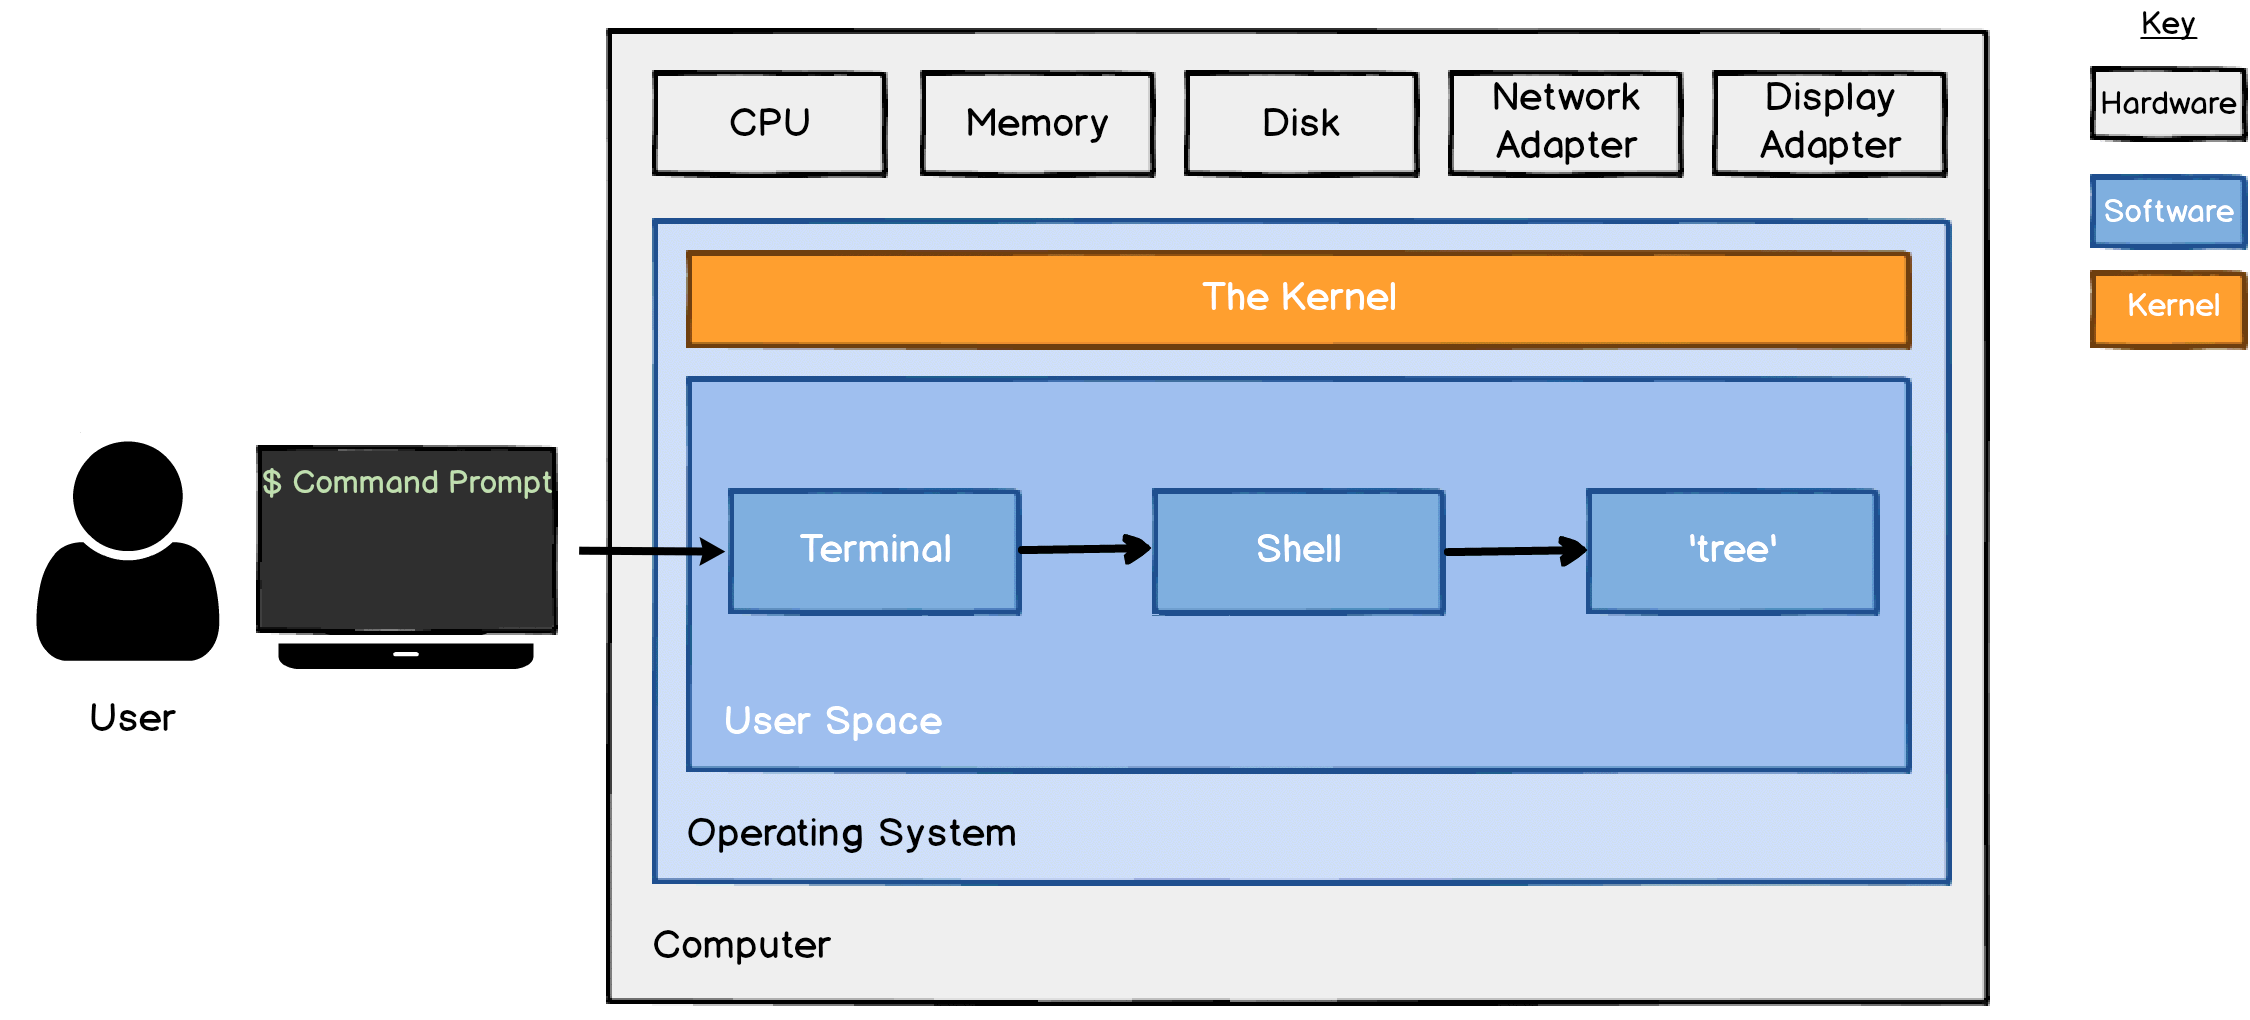
\includegraphics[width=0.8\textwidth]{assets/shell.png}
    \caption{The Shell}
    \label{fig:shell}
\end{figure}

\begin{definitionblock}[Shell]
    A shell is a program that provides the traditional, text-only user interface for Linux and other UNIX-like operating systems. Its primary function is to read commands that are typed into a console […] and then execute (i.e., run) them. The term shell derives its name from the fact that it is an outer layer of an operating system. A shell is an interface between the user and the internal parts of the OS (at the very core of which is the kernel). 
    \hfill \textit{\href{http://www.linfo.org/shell.html}{\textasciitilde Linfo}}
\end{definitionblock}

\subsection{Types of shell}

Over time, various shells have evolved to meet different needs. The most widely used is \texttt{Bash} (Bourne Again Shell), named after its creator Stephen Bourne. It's the go-to shell for most Linux systems, serving both as a command interpreter and scripting language.
Notably, macOS switched to \texttt{zsh} (Bash-compatible) from Catalina onward, while other alternatives include \texttt{Fish}, \texttt{ksh}, and \texttt{PowerShell}.

\begin{tipsblock}[Changing the Shell]
    The shell might be changed by simply typing its name and even the default shell might be changed for all sessions.
\end{tipsblock}

\subsubsection{Login vs. Non-login Shell}

A \textbf{login shell} is invoked when a user logs into the system (e.g., through a virtual terminal by pressing \texttt{Ctrl+Alt+F1}). It requires the user to provide a username and password. Once authenticated, the user is presented with an interactive shell session. Login shells are typically the first point of interaction between a user and the system.

A \textbf{non-login shell}, on the other hand, does not require the user to log in again, as it is executed within an already active user session. For example, opening a graphical terminal in a desktop environment provides a non-login (interactive) shell. Non-login shells are commonly used in environments where the user is already authenticated.

\subsubsection{Interactive vs. Non-interactive Shell}

An \textbf{interactive shell} allows users to type commands and receive immediate feedback. Both login and non-login shells can be interactive. Examples include graphical terminals and virtual terminals. In interactive shells, the prompt (\texttt{\$PS1}) must be set, which provides the user interface for command input.

A \textbf{non-interactive shell}, however, is typically executed in automated environments, such as scripts or batch processes. Input and output are generally hidden unless explicitly managed by the calling process. Non-interactive shells are usually non-login shells since the user is already authenticated. For instance, when a script is executed, it runs in a non-interactive shell. However, scripts can emulate interactivity by prompting users for input.

\section{Shell Scripting}

\subsection{Variables and Environmental Variables}

Shells, like any program, use variables to store data. Variables are assigned values using the equals sign (\texttt{=}) without spaces. For example, to assign the value \texttt{1} to the variable \texttt{A}, one would type:

\begin{codeblock}[language=bash, numbers=none]
A=1
\end{codeblock}

To retrieve a variable's value, the dollar sign (\texttt{\$}) and curly braces are used. For example:

\begin{codeblock}[language=bash, numbers=none]
echo ${A}
\end{codeblock}

Certain variables, called \textbf{environmental variables}, influence how processes run on the system. These variables are often predefined. For instance, to display the user’s home directory, use: \texttt{echo \$\{HOME\}}. To create an environmental variable, prepend the command \texttt{export}.

\begin{exampleblock}[Setting the PATH]
    For example, to add \plaintt{/usr/sbin} to the \plaintt{PATH} environmental variable:
    \begin{codeblock}[language=bash, numbers=none]
export PATH="/usr/sbin:$PATH"
    \end{codeblock}
\end{exampleblock}

The \texttt{PATH} variable specifies directories where executable programs are located, ensuring commands can be executed without specifying full paths.

When a terminal is launched, the UNIX system invokes the shell interpreter specified in the \texttt{SHELL} environment variable. If \texttt{SHELL} is unset, the system default is used. After sourcing initialization files, the shell presents the prompt, which is defined by the \texttt{\$PS1} environment variable.

\subsection{Initialization Files}

Initialization files are scripts or configuration files executed when a shell session starts. They set up the shell environment, define default settings, and customize behavior. Depending on the type of shell (login, non-login, interactive, or non-interactive), different initialization files are sourced.

\begin{itemize}
    \item \textbf{Login Shell Initialization Files}:
    \begin{itemize}
        \item Bourne-compatible shells: \texttt{/etc/profile}, \texttt{/etc/profile.d/*}, \texttt{\textasciitilde/.profile}.
        \item Bash: \texttt{\textasciitilde/.bash\_profile} (or \texttt{\textasciitilde/.bash\_login}).
        \item zsh: \texttt{/etc/zprofile}, \texttt{\textasciitilde/.zprofile}.
        \item csh: \texttt{/etc/csh.login}, \texttt{\textasciitilde/.login}.
    \end{itemize}

    \item \textbf{Non-login Shell Initialization Files}:
    \begin{itemize}
        \item Bash: \texttt{/etc/bash.bashrc}, \texttt{\textasciitilde/.bashrc}.
    \end{itemize}

    \item \textbf{Interactive Shell Initialization Files}:
    \begin{itemize}
        \item \texttt{/etc/profile}, \texttt{/etc/profile.d/*}, and \texttt{\textasciitilde/.profile}.
        \item For Bash: \texttt{/etc/bash.bashrc} and \texttt{\textasciitilde/.bashrc}.
    \end{itemize}

    \item \textbf{Non-interactive Shell Initialization Files}:
    \begin{itemize}
        \item For Bash: \texttt{/etc/bash.bashrc}. 
        
        However, most scripts begin with the condition \texttt{[ -z "\$PS1" ] \&\& return}.
        This means that if the shell is non-interactive (as indicated by the absence of the \texttt{\$PS1} prompt variable), the script stops execution immediately.
        
        \item Depending on the shell, the file specified in the \texttt{\$ENV} (or \texttt{\$BASH\_ENV}) environment variable may also be read.
    \end{itemize}
\end{itemize}

\subsection{Basic Shell Commands}

To become familiar with the shell, let’s start with some fundamental commands:

\begin{itemize}
    \item \texttt{echo}: Prints the text or variable values you provide at the shell prompt.
    \item \texttt{date}: Displays the current date and time.
    \item \texttt{clear}: Clears the terminal screen.
    \item \texttt{pwd}: Stands for \textit{Print Working Directory}, showing the current directory the shell is operating in. It is also the default location where commands look for files.
    \item \texttt{ls}: Stands for \textit{List}, and lists the contents of the current directory.
    \item \texttt{cd}: Stands for \textit{Change Directory}, and switches the current directory to the specified path.
    \item \texttt{cp}: Stands for \textit{Copy}, and duplicates files or directories from a source to a destination.
    \item \texttt{mv}: Stands for \textit{Move}, and transfers files or directories from one location to another. It can also rename files.
    \item \texttt{touch}: Creates a new, empty file or updates the timestamps of an existing file.
    \item \texttt{mkdir}: Stands for \textit{Make Directory}, and creates new directories.
    \item \texttt{rm}: Stands for \textit{Remove}, and deletes files or directories. To delete directories, the recursive option (\texttt{-r}) must be used.
\end{itemize}

\begin{warningblock}[Remove Command]
    Be cautious when using the \plaintt{rm} command, as it permanently deletes files and directories \textbf{without moving them to the trash}.
\end{warningblock}

\subsection{Shell Scripts}

Commands can be written in a script file, which is a text file containing instructions for the shell to execute. 
The first line of the script, known as the \textbf{shebang}, specifies the interpreter to use.

\begin{codeblock}[language=bash, numbers=none]
#!/bin/bash
#!/usr/bin/env python
\end{codeblock}

To make a script executable, you need to change its permissions:
\texttt{chmod +x script\_file}

\subsubsection{Not All Commands Are the Same}

Commands in the shell can behave differently depending on how they are executed. For example, when a command like \texttt{ls} is run, it creates a \textbf{subprocess}, a separate instance that inherits the environment of the parent shell. This subprocess runs the command and then terminates, returning control to the parent shell.

\begin{tipsblock}[Running Commands]
    \begin{itemize}
        \item \textbf{Subprocess}: Subprocesses can't modify the parent shell's environment or state. Changes made in subprocesses don't persist.
        \item \textbf{\plaintt{source}}: The \plaintt{source} command (or \plaintt{.}) runs scripts in the current shell context, allowing environment modifications.
        \item \textbf{Scripts}: Running with \plaintt{./script\_file} creates a subprocess, isolating effects from the parent shell.
    \end{itemize}
\end{tipsblock}

\subsubsection{Types of Commands}

In the shell, commands can fall into several categories:

\begin{itemize}
    \item \textbf{Built-in Commands}: These are commands provided directly by the shell, such as \texttt{cd}, that are executed without creating a subprocess, necessary to update environment variables.
    \item \textbf{Executables}: These are standalone programs stored in directories specified by the \texttt{\$PATH} environment variable. Examples include \texttt{ls}, \texttt{grep}, and \texttt{find}.
    \item \textbf{Functions and Aliases}: These are user-defined commands or shortcuts, often configured in initialization files like \texttt{\textasciitilde/.bashrc}.
\end{itemize}

To determine the type of a command and its location you can use:
\begin{itemize}
    \item \texttt{type command\_name} to identify if the command is built-in, an executable, or a function/alias.
    \item \texttt{which command\_name} to find the exact location of an executable in the file system.
\end{itemize}

\newpage

\begin{warningblock}[Spaces in File Names]
    Avoid using spaces or accented characters in file names. Instead, use:
    \begin{itemize}
        \item \plaintt{my\_file\_name} (snake case),
        \item \plaintt{myFileName} (camel case),
        \item \plaintt{my-file-name} (kebab case).
    \end{itemize}
    Spaces complicate scripts and make parsing error-prone.
\end{warningblock}

\subsection{Functions}

A \textbf{function} in a shell script is a reusable block of code. The syntax is:
\begin{codeblock}[language=bash]
function_name() {
    # Commands to execute
}
\end{codeblock}

Scripts or functions can access \textbf{input arguments} passed to them using special variables:
\begin{itemize}
    \item \texttt{\$0}: The name of the script or function.
    \item \texttt{\$1}, \texttt{\$2}, \texttt{\$3}, etc.: The first, second, third, etc., arguments.
    \item \texttt{\$\#}: The number of arguments passed.
    \item \texttt{\$@}: All arguments as separate words.
    \item \texttt{\$*}: All arguments as a single word (rarely used).
\end{itemize}

\begin{exampleblock}[Sum Function]
    An example function that prints the sum of two numbers:
    \begin{codeblock}[language=bash]
sum() {
    echo $(($1 + $2))
}
    \end{codeblock}
\end{exampleblock}

\subsection{Additional Shell Commands}

\subsubsection{More Commands}

\begin{itemize}
    \item \texttt{cat}: Stands for \textit{Concatenate}. Reads and outputs the contents of files. It can read multiple files and concatenate their content.
    \item \texttt{wc}: Short for \textit{Word Count}. Provides statistics like newline count, word count, and byte count for a list of files.
    \item \texttt{grep}: Stands for \textit{Global Regular Expression Print}. Searches for lines containing a specific string or matching a given pattern.
    \item \texttt{head}: Displays the first few lines of a file.
    \item \texttt{tail}: Displays the last few lines of a file.
    \item \texttt{file}: Examines specified files to determine their type.
\end{itemize}

\subsubsection{Redirection, Pipelines, and Filters}

Commands can be combined using operators to manipulate input and output streams:
\begin{itemize}
    \item The \textbf{pipe operator} (\texttt{|}) forwards the output of one command to another.
    
    Example: \texttt{cat /etc/passwd | grep <word>} filters system information for a specific word.
    
    \item The \textbf{redirect operator} (\texttt{>}) sends the standard output to a file.
    
    Example: \texttt{ls > files-in-this-folder.txt}.
    
    \item The \textbf{append operator} (\texttt{>>}) appends output to an existing file.
    \item The \textbf{operator} (\texttt{\&>}) redirects both standard output and standard error to a file.
    \item \textbf{Logical operators}:
    \begin{itemize}
        \item \texttt{\&\&}: Executes the next command only if the previous one succeeds.
        
        Example: \texttt{sudo apt update \&\& sudo apt upgrade}.
        
        \item \texttt{||}: Executes the next command only if the previous one fails.
        \item \texttt{;}: Executes commands sequentially, regardless of the status of the previous command.
    \end{itemize}
    \item \texttt{\$?}: Contains the exit status of the last command.
\end{itemize}

\subsubsection{Advanced Commands}

\begin{itemize}
    \item \texttt{tr}: Stands for \textit{Translate}. Performs character transformations.
    \begin{itemize}
        \item Example: \texttt{echo "abc" | tr [a-z] [A-Z]} converts lowercase to uppercase.
        \item Example: \texttt{echo "123abc" | tr -d [:digit:]} removes digits.
    \end{itemize}
    \item \texttt{sed}: A \textit{stream editor} for text processing.
    \begin{itemize}
        \item Example: \texttt{echo 'UNIX is great' | sed 's/UNIX/Linux/'} replaces 'UNIX' with 'Linux'.
        \item Example: \texttt{echo "1\textbackslash{}n2\textbackslash{}n3" | sed "2d"} deletes the second line.
    \end{itemize}
    \item \texttt{cut}: Extracts specific sections from lines of text.
    \begin{itemize}
        \item Example: \texttt{cut -b 1-3 file.txt} extracts the first three bytes of each line.
        \item Example: \texttt{echo "1,2,3" | cut -d "," -f 1} retrieves the first column.
    \end{itemize}
    \item \texttt{find}: Searches for files based on conditions.
    
    Example: \texttt{find . -type d -name "*lib*"} searches for directories containing "lib".

    \item \texttt{locate}: Faster alternative to \texttt{find}, relying on a pre-built database. Update the database with \texttt{updatedb}.
    
    Example: \texttt{locate -i foo} finds items containing "foo", ignoring case.
\end{itemize}

\subsubsection{Quoting in Shell}

Quoting affects how strings and variables are interpreted:
\begin{itemize}
    \item \texttt{""}: Double quotes interpret variables.
    \item \texttt{''}: Single quotes treat everything as literal.
\end{itemize}

\begin{exampleblock}[Quoting]
    \begin{codeblock}[language=bash]
a=yes
echo "\$a" # Outputs "yes".
echo '\$a' # Outputs "\$a".
    \end{codeblock}
\end{exampleblock}

The output of a command can be converted into a string and assigned to a variable for later reuse: 

\begin{neonlisting}[language=bash]{Output conversion}
list=$(ls -l) 
# or equivalently:
list=`ls -l`
\end{neonlisting}

\subsubsection{Processes}

Managing background and foreground processes:
\begin{itemize}
    \item \texttt{./my\_command \&}: Run a command in the background.
    \item \texttt{Ctrl-Z}: Suspend the current process.
    \item \texttt{jobs}: List background processes.
    \item \texttt{bg \%n}: Resume a suspended process in the background.
    \item \texttt{fg \%n}: Bring a background process to the foreground.
    \item \texttt{Ctrl-C}: Terminate the foreground process.
    \item \texttt{kill pid}: Send a termination signal to a process.
    \item \texttt{ps aux | grep process}: Find running processes.
\end{itemize}

Processes in the background are terminated when the terminal closes unless started with \texttt{nohup}.

\begin{tipsblock}[How to Get Help]
    \begin{itemize}
        \item \plaintt{command -h} or \plaintt{command --help}: Display a brief help message.
        \item \plaintt{man command}: Access the manual for the command.
        \item \plaintt{info command}: Show detailed information (if available).
    \end{itemize}
\end{tipsblock}